Since SEOSS Dataset\cite{RATH2019104005} was only evaluated and trained with SQLNet and RatSQL in this section, we decided to investigate further by experimenting with this dataset using state-of-the-art solutions currently proposed for the SPIDER challenge. In order to determine the effectiveness of these methods, we compared the results obtained with those of SQLNet\ref{sec:sqlnet} and RatSQL\ref{sec:ratsql} from the SEOSS-Queries research paper\cite{TOMOVA2022108211}. The results of these experiments are presented in the following section, and they will demonstrate the potential of modern solutions for solving the SPIDER task.

\subsection{Limitations}

Our experiment requires a lot of computational resources as we mainly leverage the T5 model. We used a single Nvidia RTX 3070 16GB GPU with 40GB Memory for our experiment, which unfortunately limited us to smaller models with more restrictions. Despite these limitations, we were still able to achieve excellent results. If we had used a larger T5 model, such as T5-3B, we would have been able to reach much higher scores. Therefore, investing in a more powerful GPU for our experiment is something that we must consider in order to maximize our results.

\subsection{SEOSS + T5 PICARD Experiment}
After studying the SEOSS dataset, we decided to experiment with the PICARD model\ref{picard} to evaluate its performance against that of SQLNet and RatSQL. We decided to use the T5Base model for our experiment, as it is smaller than the T5-3B and T5-11B models used by most state-of-the-art studies. To ensure a fair comparison between the models, we used two beam sizes of 2 and 4 and the same evaluation metrics as SEOSS-SQLNet and SEOSS-RatSQL, which is "exact matching accuracy". We wanted to see if the PICARD model could achieve similar results to those of SQLNet and RatSQL, so we conducted our experiment with our findings. The results of our experiment are discussed in the following section and can be used to compare the performance of the PICARD model to the models used in the SEOSS study.
\footnote[1]{Link to the Github Page: \url{https://github.com/yazdipour/text-to-sql-seoss-t5}}

\begin{table}[!ht]
    \centering
    \begin{tabular}{|c|c|c|L|L|}
        \hline
        Model    & Picard Mode       & Beams & \textbf{Exact Matching Accuracy} & \textbf{Execution Accuracy} \\ \hline
        T5-base  & parse with guards & 2     & 0.3297                           & 0.3576                      \\ \hline
        T5-base  & lex               & 4     & 0.3071                           & 0.3039                      \\ \hline
        T5-base  & parse with guards & 4     & 0.3286                           & 0.3512                      \\ \hline
        T5-large & parse with guards & 4     & 0.4274                           & 0.4822                      \\ \hline
    \end{tabular}
    \caption{Expermiment Accuracy Results}
\end{table}

The table shows the results of various configurations of T5-base and T5-large models for natural language processing tasks. The configurations are differentiated by the Picard mode parse with guards or lex and the number of beams used in the beam search process 2 or 4.

Comparing the results, we can observe that:
\begin{itemize}
    \item The T5-large model generally performs better than the T5-base model in both exact matching accuracy and execution accuracy.
    \item The parse with guards Picard mode performs better than the lex Picard mode in both models.
    \item Using four beams instead of 2 in the beam search process improves the performance for both models and Picard modes.
    \item The highest exact matching accuracy is achieved by the T5-large model with parse with guards Picard mode and four beams 0.4274.
    \item The highest execution accuracy is also achieved by the T5-large model with parse with guards Picard mode and four beams 0.4822.
    \item Increasing beam size does not have a significant effect compared to changing the model and mode.
\end{itemize}


\begin{table}[h]
    \centering
    \begin{tabular}{|c|c|c|c|c|c|}
        \hline
        \multirow{2}*{Exact Match Accuracy} & easy  & medium & hard  & extra hard & all   \\
                                            & 392   & 378    & 77    & 84         & 931   \\ \hline
        SQLNet                              & 0.023 & 0.000  & 0.000 & 0.000      & 0.010 \\ \hline
        RatSQL + Glove                      & 0.309 & 0.214  & 0.091 & 0.000      & 0.224 \\ \hline
        RatSQL + Bert                       & 0.161 & 0.201  & 0.065 & 0.012      & 0.156 \\ \hline
        PICARD + T5Base + 4Beam             & 0.446 & 0.254  & 0.182 & 0.012      & 0.307 \\ \hline
        PICARD + T5Large + 4Beam            & 0.571 & 0.410  & 0.182 & 0.060      & 0.427 \\ \hline
    \end{tabular}
    \caption{Comparison between Exact Match Accuracy}
\end{table}

The table compares the exact match accuracy of various models that are not fine-tuned for our dataset. The models are evaluated on five difficulty levels: easy, medium, hard, extra hard, and all.

Comparing the results, we can observe that:
\begin{itemize}
    \item The PICARD + T5Large + 4Beam model has the highest exact match accuracy among all models and difficulty levels, with a maximum value of 0.571; this shows that this model is more generalized and can handle unseen databases quite well compared to other solutions.
    \item The PICARD + T5Base + 4Beam model performs better than the other models, with a maximum value of 0.446.
    \item The RatSQL models with Glove and Bert embeddings perform similarly, with a maximum value of 0.309 and 0.201, respectively.
    \item The SQLNet model performs the worst among all models, with a maximum value of 0.023.
    \item The extra hard and all difficulty levels generally have lower exact match accuracy values compared to the easy and medium levels. Amazingly T5 PICARD was still able to solve complex problems with a low percentage, yet better than the other models.
    \item Research in\cite{TOMOVA2022108211} shows that the trained RatSQL were able to achieve a high exact match accuracy. This is a good sign that the PICARD model can achieve high accuracy with a little fine-tuning.
\end{itemize}

\subsection{Recall and F1 Scores}

Here, we can observe the Recall and F1 scores of each SQL Keyword for the PICARD T5-Large 4-Beam experiment on the SEOSS dataset. We can see that PICARD has managed to attain a very impressive F1 score for the SEOSS dataset without even having to be specifically trained for our dataset. This is a very encouraging result and indicates that the model is able to generalize accurately across different domains. Moreover, it is essential to note that the F1 score obtained by the PICARD model was obtained without any additional fine-tuning. This is a testament to the robustness and capability of the model and further highlights its ability to generalize to different datasets.

We experimented with a variety of different parameters, including beam size, modes and model sizes, and spent multiple hours for each evaluation. These experiments have been carefully documented in the Appendix\ref{sec:appendix} of this thesis, where you can find the results in detail.


% \begin{table}[h]
%     \centering
%     \begin{tabular}{|c|c|c|c|c|c|}
%         \hline
%                          & easy  & medium & hard  & extra & all   \\ \hline
%         select           & 0.709 & 0.585  & 0.390 & 0.440 & 0.608 \\ \hline
%         select(no AGG)   & 0.709 & 0.590  & 0.390 & 0.452 & 0.611 \\ \hline
%         where            & 0.708 & 0.520  & 0.200 & 0.273 & 0.523 \\ \hline
%         where(no OP)     & 0.750 & 0.526  & 0.200 & 0.325 & 0.548 \\ \hline
%         group(no Having) & 0.429 & 0.754  & 0.914 & 0.286 & 0.691 \\ \hline
%         group            & 0.000 & 0.726  & 0.914 & 0.214 & 0.649 \\ \hline
%         order            & 0.000 & 0.143  & 0.543 & 0.310 & 0.343 \\ \hline
%         and/or           & 0.987 & 0.997  & 1.000 & 0.983 & 0.992 \\ \hline
%         keywords         & 0.823 & 0.725  & 0.649 & 0.417 & 0.704 \\ \hline
%     \end{tabular}
%     \caption{Partial Matching Recall - PICARD T5-Large 4-Beam}
% \end{table}

% add image here pics/ez/Recall.png
% \begin{figure}[h]
%     \centering
%     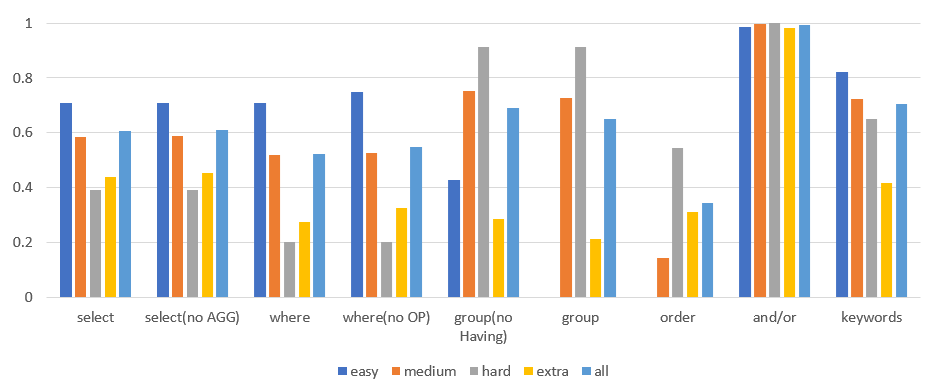
\includegraphics[width=0.8\textwidth]{pics/ez/Recall.png}
%     \caption{Partial Matching Recall - PICARD T5-Large 4-Beam}
% \end{figure}

% \begin{table}[h]
%     \centering
%     \begin{tabular}{|c|c|c|c|c|c|}
%         \hline
%                          & easy  & medium & hard  & extra & all   \\ \hline
%         select           & 0.743 & 0.625  & 0.395 & 0.490 & 0.644 \\ \hline
%         select(no AGG)   & 0.743 & 0.631  & 0.395 & 0.503 & 0.647 \\ \hline
%         where            & 0.723 & 0.593  & 0.230 & 0.323 & 0.576 \\ \hline
%         where(no OP)     & 0.766 & 0.599  & 0.230 & 0.385 & 0.604 \\ \hline
%         group(no Having) & 0.214 & 0.770  & 0.889 & 0.369 & 0.705 \\ \hline
%         group            & 1.000 & 0.741  & 0.889 & 0.277 & 0.661 \\ \hline
%         order            & 1.000 & 0.182  & 0.535 & 0.394 & 0.393 \\ \hline
%         and/or           & 0.994 & 0.971  & 0.908 & 0.817 & 0.964 \\ \hline
%         keywords         & 0.809 & 0.781  & 0.690 & 0.483 & 0.746 \\ \hline
%     \end{tabular}
%     \caption{Partial Matching F1 - PICARD T5-Large 4-Beam}
% \end{table}

% add image here pics/ez/F1.png
\begin{figure}[h]
    \centering
    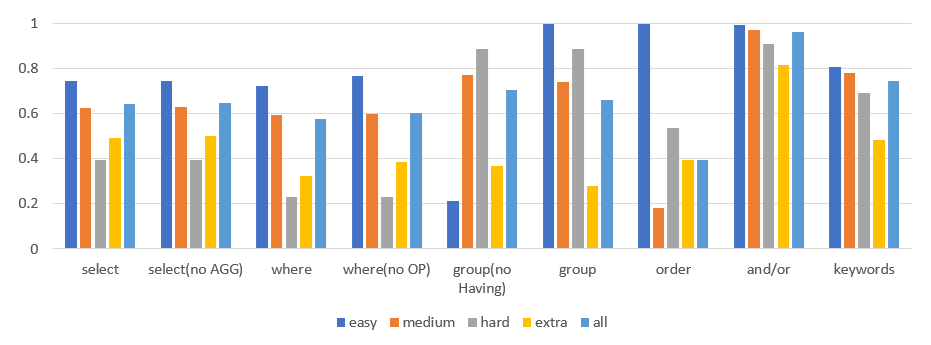
\includegraphics[width=1\textwidth]{pics/ez/F1.png}
    \caption{F1 Scores of Component Matching - PICARD T5-Large 4-Beam}
\end{figure}
